\section{Implementation Details}
\label{ch:implementation}

The following is a discussion of how HCCP works at an implementation level.
Since HCCP is designed to be run on different hardware, with
different capabilities, it is best to describe the network
setup in terms of communication. Specifics about mote design,
real-time operating systems and communication stacks are abstracted. 


\subsection{Clusterhead Election}


HCCP takes a different approach than LEACH to electing clusterheads.
Motes can't just be cluster members, even though being a clustermote every round
is the most energy-efficient thing to do. 
A problem inadvertently created by HCCP's attempt to allow more motes
be clustermembers, is that if a mote is by a sink, it would never choose to be a clusterhead. 
In the Clusterhead Candidacy phase, the sink will always broadcast first, never allowing
motes in range of the sink to be clusterheads, since they would always concede to the sink.
%If motes never became clustermotes due to there being a very good 
%clusterhead next to them, there would be an invisible wall around the 
%sink of motes that never become clusterheads. 
Since no motes
around the sink would ever be clusterheads,
motes out of range of the sink cannot hop messages to the sink. This would create an invisible wall around the sink, where motes past
the wall will never have messages reach the sink. If a mote does not complete any messages, it is
suffering starvation, a term taken from task scheduling in operating systems when processes will never run due
to higher priority processes continually running.
The effects of starvation can be seen in Figures~\ref{fig:images_HCCPBlocking_hccpblocking} and~\ref{fig:starvationMap}.
Figure~\ref{fig:images_HCCPBlocking_hccpblocking} shows a comparison of distance from the sink to how many messages have been 
received at the sink, and it is clear that no messages beyond 100 arbitrary distance units from the sink would ever have 
messages received at the sink.
Figure~\ref{fig:starvationMap} shows a map of where the motes are that have completed messages, and which motes are 
suffering from starvation (the sink is the green triangle in the middle of the network).
A few messages from motes beyond the invisible wall can be received at the base station if
collisions in clusterhead candidacy messages, allowing motes within the invisible wall to become clusterheads. Motes that 
did not get that message could then elect to be a clusterhead, allowing messages in 
from beyond the wall. Starvation does not happen in LEACH since the clusterhead elections happen 
independent of each other, as shown in Figure~\ref{fig:StarvationLeach} which is created from the 
same network with the same configuration settings using LEACH as an election protocol. 
Therefore, a solution is needed to avoid creating the invisible wall that 
the Clusterhead Candidacy phase has created.

\begin{figure}[htb]
	\centering
		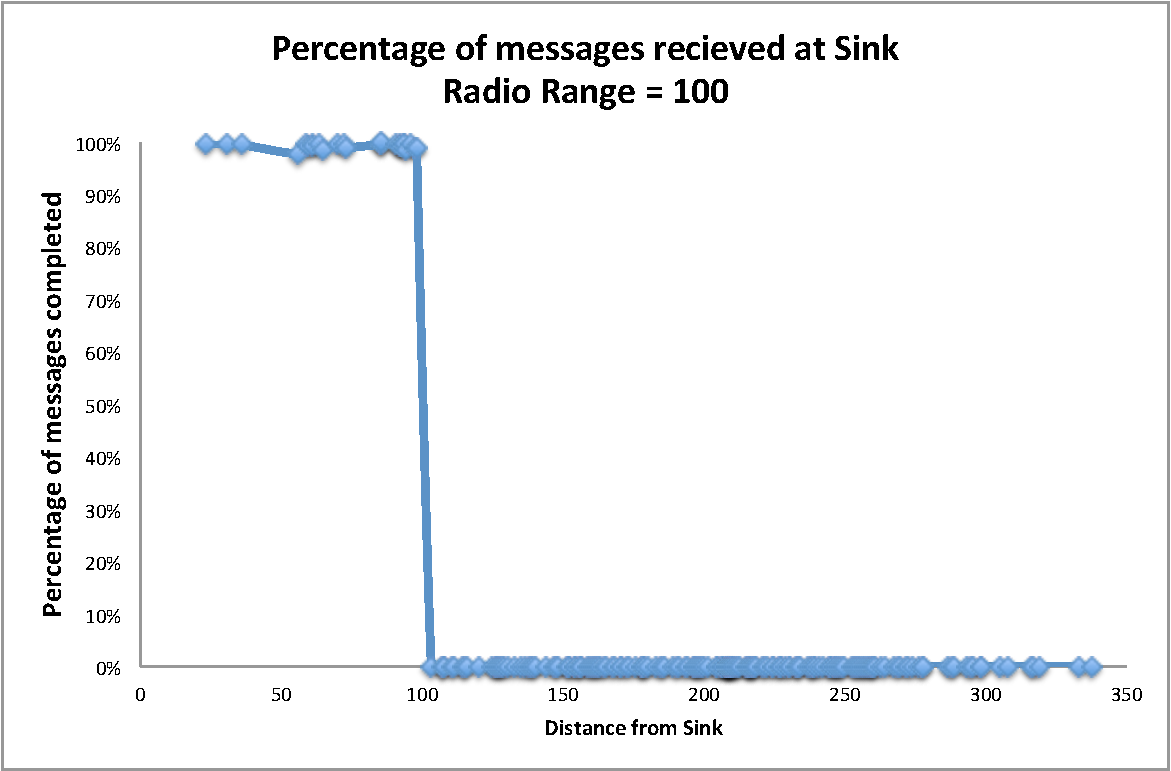
\includegraphics[height=3in]{images/HCCPBlocking/starvation.pdf}
	\caption{An invisible wall created due to HCCP clusterhead candidacy messages.}
	\label{fig:images_HCCPBlocking_hccpblocking}
\end{figure}
\begin{figure}[htb]
	\centering
		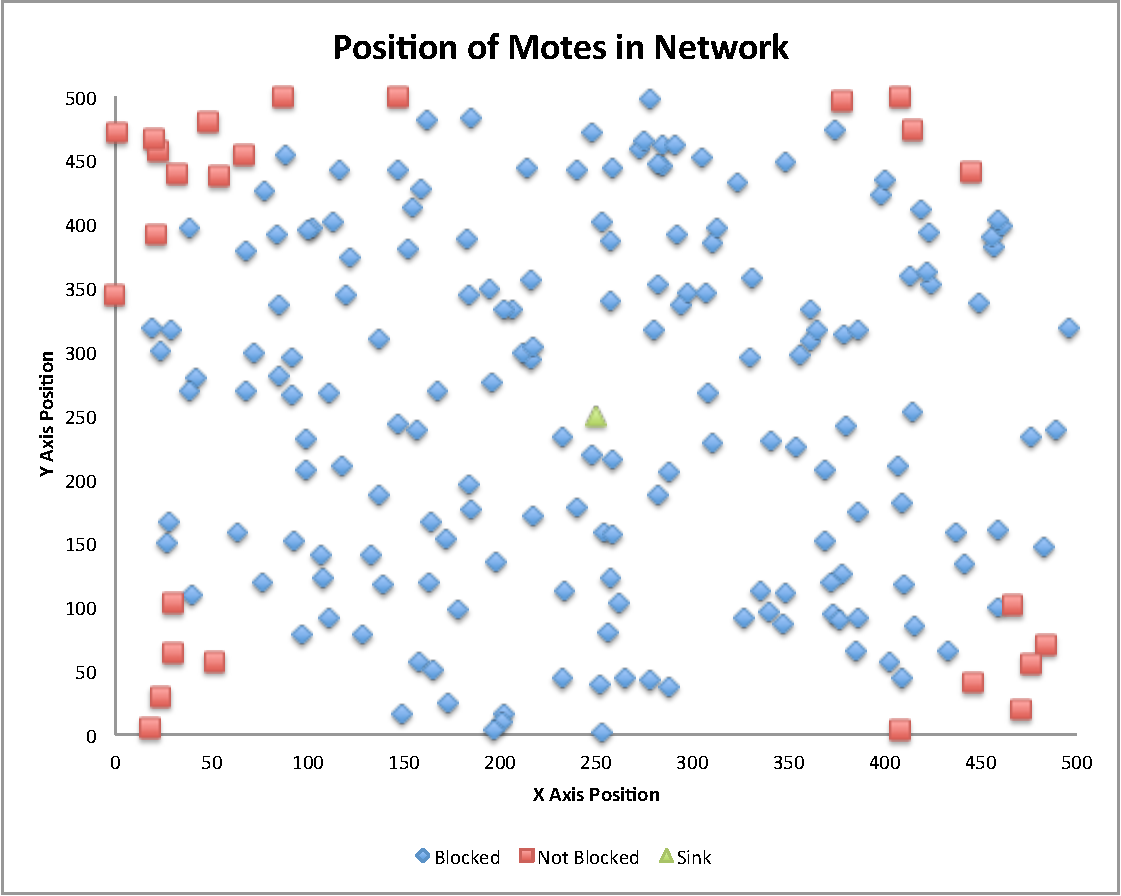
\includegraphics[height=3.5in]{images/HCCPBlocking/starvationMap.pdf}
	\caption{HCCP messages received at the base station. There is no way messages outside the radio range of the sink can send messages to the sink.}
	\label{fig:starvationMap}
\end{figure}

\begin{figure}[htb]
	\centering
		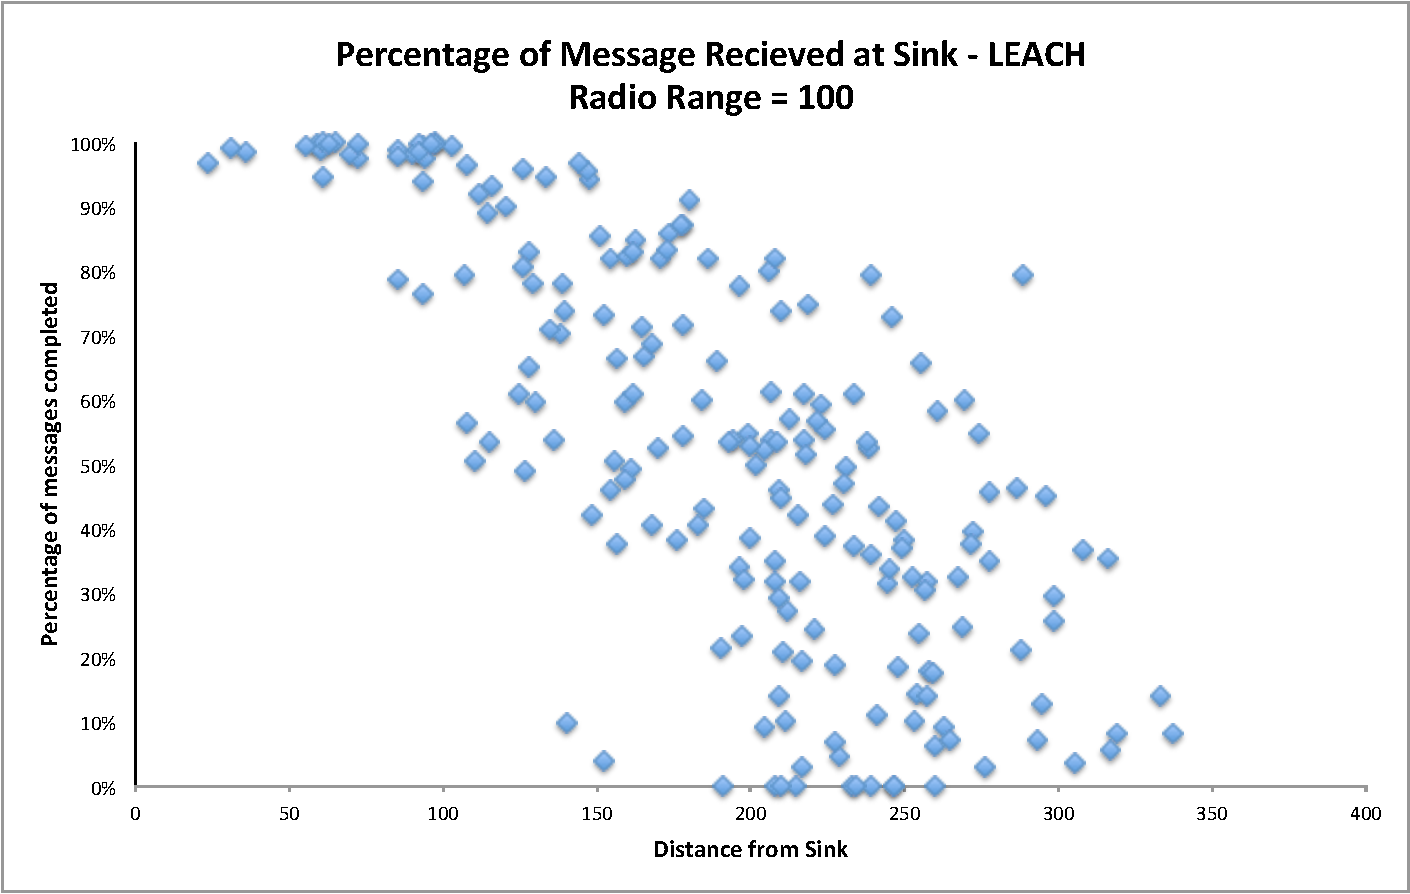
\includegraphics[height=3in]{images/HCCPBlocking/StarvationLeach.pdf}
	\caption{LEACH messages reached at the base station, note there is no `wall' blocking messages.}
	\label{fig:StarvationLeach}
\end{figure}

There are two different approaches to eliminate the problem of the `invisible wall' in HCCP.
\begin{enumerate}
\item The sink can sleep for a cycle. Since the sink would not send a
clusterhead candidacy message, the surrounding motes would then 
be able to become clusterheads. This would allow messages to flow into the 
motes in range of the sink from motes out of range of the sink.
\item Motes can choose to be clusterheads \emph{even if} there is a better clusterhead in range.
Since the sink will always be a better clusterhead than a mote, a mote should 
be able to ignore all other candidacy messages and become a clusterhead.
\end{enumerate}


Both of these have drawbacks. If the sink turns off for a cycle, the latency time for messages
will go up, since no messages will be received at the sink for this time. If clusterheads
are allowed to randomly choose to be clusterheads, there will be more collisions
due to the increased number of messages being sent during clusterhead messaging times (clusterhead
elections and the like).

To discover which of these methods is better to  use, a simulation of both LEACH and HCCP 
was created and the results were compared, and are compared later in section~\ref{sleepVSsubop}.


\subsection{HCCP Goodness Delay}
\label{subsec:goodnessDelay}
%The better I am, the sooner I announce it.

To ensure that motes that are better at being clusterheads are chosen to be clusterheads, the timing that
is inherent in an election/run WSN such as LEACH is leveraged.  If a mote has the right qualifications
for being a good clusterhead, it announces its candidacy first. If another mote that was
going to announce its clusterhead candidacy hears the a different mote's candidacy message first,
it will not be a clusterhead that round. 

The Goodness Delay is created by delaying a percentage of the available time. 
%is derived by a `percentage of goodness' 
Motes that are well suited for being a clusterhead will create a small delay (therefore
announcing itself as a potential clusterhead earlier), and motes that are not well suited for being 
a clusterhead will have longer delays.

Since the heterogeneous assessment can focus on different heterogeneous factors,
the way of determining how long to delay must be robust to the possible focuses.
To reflect this, a percentage of time to delay is put into a weighted average of
all the factors that will contribute to the delay timing.
The code looks like the following:

{\ssp \vskip 1em  \hangindent=0.5cm
\lstset{basicstyle=\footnotesize\ttfamily,language=Java}
\begin{lstlisting}
private double getGoodnessDelay()
{
  double delay = 0;

  // add up to n% of available time based on battery
  delay =  (availableTime * BATTERY_POWER_WEIGHT  * 
      (1 - battery.getPercentLeft() ) );

  // n% of available time based on mission
  // delay gets longer if this node wants to be a clustermote
  delay = delay + (availableTime * SENSOR_MISSION_WEIGHT *
       sensorMission );

  // n% on messagequeue size
  delay = delay + (availableTime * MESSAGE_QUEUE_WEIGHT * 
      ( messageQueue.size()/(double)maxQueueSize ) );

  // n% of random
  delay = delay + (availableTime * RANDOM_WEIGHT * 
      (goodnessRM.nextDouble()));

  // n% of duty cycling based on last round as CH.
  // more delay if I was just a clusterhead.
  delay = delay + (availableTime * DUTY_CYCLE_WEIGHT *  
      ( 1- Math.min(1, lastRoundAsClusterhead * chanceOfBeingCH)));

  return delay;
}
\end{lstlisting}
}


 \subsubsection{Continuous Nature of HCCP Goodness Delay}
     Since HCCP uses a Goodness Delay to advertise the heterogeneity of the network, it can be considered
     a continuous statistic. This is as opposed to the two/three/n-tier network that describes a network
     as a binary relationship between motes: a mote is a routing mote or not. HCCP takes what is known about 
     the mote, and translates that information into a continuous distribution via the Goodness Delay algorithm.
     The Goodness Delay calculates a percentage of `Goodness as clusterhead', and maps that Goodness to an amount
     of time to delay before becoming a clusterhead. Therefore, HCCP considers every mote to be a heterogeneous mote,
     even in a homogeneous network. Even in a homogeneous network, not all motes will be the same. Some motes will have 
     batteries that are drained more than others, and some will have no space in their message queue to become a clusterhead.
     This approach considers such factors.
     
     
 \subsubsection{Drawbacks to Goodness Delay}
     When a network is first deployed, all motes will have full batteries, empty message queues and 
     will generate approximately the same Goodness Delay.
     This would cause the Clusterhead Candidacy and Clusterhead Election time to effectively only be in the first 10th or so of the 
     time allotted to the stage.
     
     \begin{figure}[t]
      	\centering
      		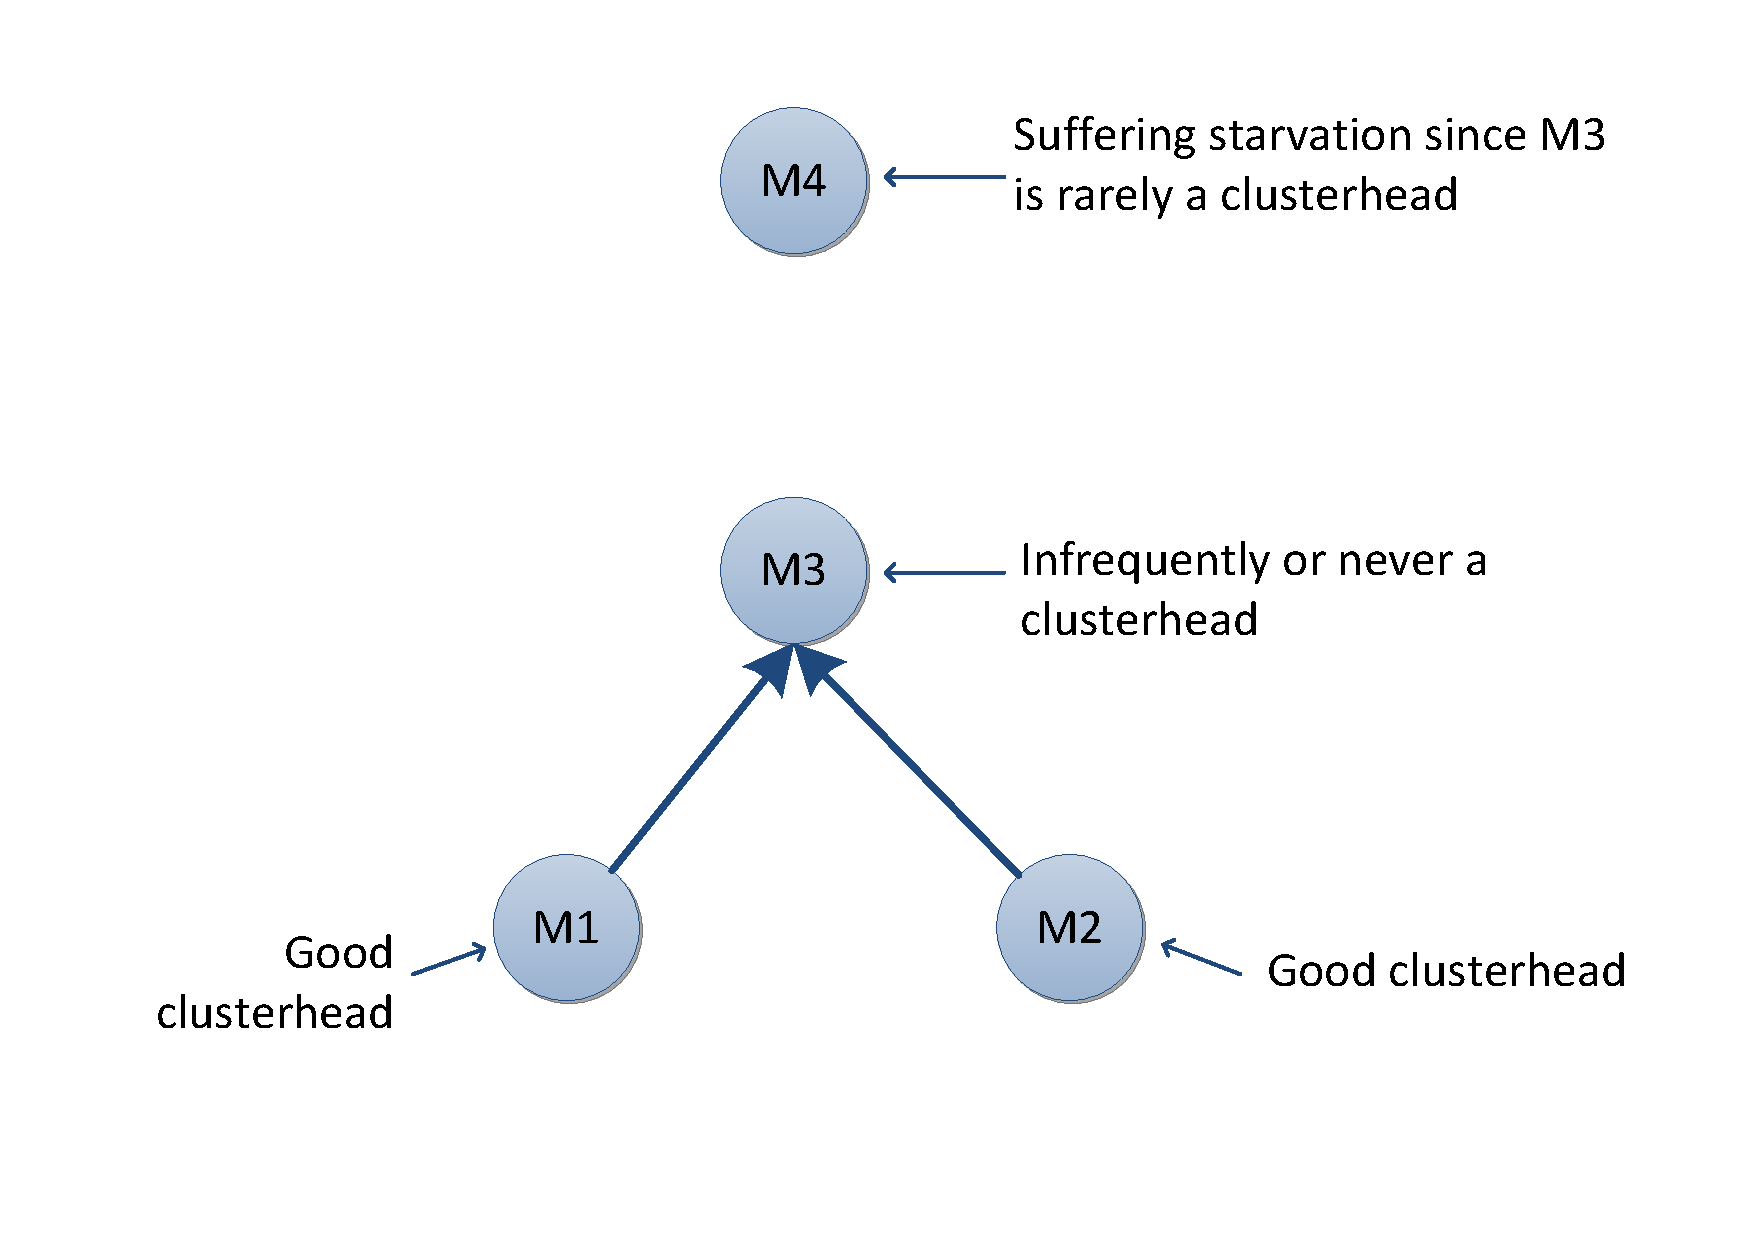
\includegraphics[height=3in]{images/HCCPBlocking/hiddenNode/BetterHiddenNode.pdf}
      	\caption{M3 never becomes a clusterhead since M1 and M2 announce their Clusterhead Candidacy first. Since M3 is never a clusterhead, M4 never has a chance to send its messages through the network.}
      	\label{fig:images_HCCPBlocking_hiddenNode_HiddenNode}
      \end{figure}
     
     
     Conversely, if motes are added to the network after it has run for a while, the HCCP Goodness Delay
     will use much more of the stage time to announce clusterheads, since the new motes will have new batteries and
     empty message queues and therefore have short Goodness Delays, while the old motes will have longer
     Goodness Delays. Due to this, HCCP is very robust to changes after the network has been run for any amount of time.



     
\subsubsection{Suboptimal Clusterheads}
\label{hccp_blocking}

Suboptimal clusterheads are crucial to the success of a network. Starvation can occur in any 
place in the network if a mote is surrounded by other motes that are also poor clusterheads, 
as shown in Figure~\ref{fig:images_HCCPBlocking_hiddenNode_HiddenNode}. Surrounding motes are 
never clusterheads since the surrounding nodes are in radio range of a good clusterhead. The
good clusterhead will advertise itself as a clusterhead, which stops all surrounding motes 
from becoming clusterheads. Since all the surrounding motes are always clustermotes, messages never leave
the mote suffering from starvation. Since this starvation can take place anywhere in the network, it could
be called in-network starvation.

To avoid in-network starvation, all motes should occasionally become clusterheads, even if 
the mote is not well-suited to becoming a clusterhead. Since the mote is not well-suited to being
a clusterhead, this is called becoming a suboptimal clusterhead. Suboptimal clusterheads prevent
in-network starvation by becoming a clusterhead to a mote that is suffering in-network starvation; collecting 
its messages and hopping the messages through the network. 

Due to the timed nature of HCCP elections, suboptimal clusterheads will announce their
candidacy later than good clusterheads. Since the announcement is later, only motes that are suffering
starvation or have no better options (better being defined as a clusterhead that announces earlier or has a lower beacon rank for routing) 
will choose to follow the suboptimal clusterhead. This means that cluster sizes for suboptimal clusterheads should 
be smaller than a normal cluster size. 
If HCCP did not use a timed election, then the cluster for the suboptimal clusterhead's cluster may get too large, sending
too many messages and overrun
the clusterhead's message queue (too many messages received from the cluster), therefore wasting more energy
than needed to 
be a clusterhead.



\subsubsection{Suboptimal First-order Clusterheads}

Since the sink can be considered to be a clusterhead, and is a clusterhead for each round, the motes in radio range of the sink
(called first-order clusterheads)
should be given a different rate of choosing to be a suboptimal clusterhead. A first-order clusterhead is a clusterhead 
that has a beacon rank of 1, that is, is within radio range of the sink.

Since all messages need to be hopped through the motes that are next to the sink, they need to spend more time 
as clusterheads. This is so the first-order clusterheads can receive messages from the rest of the network and 
relay them to the sink.

\subsubsection{Sink Sleep}

Another solution to getting messages to the first-order motes, is to turn
the sink off for a round. Turning the sink off will allow the first-order
motes to become clusterheads. Allowing the first-order motes to be clusterheads
will allow the messages from the network to flow into the first-order motes. Once the 
messages have flowed into the first-order motes, the messages can easily be hopped to the sink.



\subsection{Roundtable Discussion Functions}

As networks were simulated, it was obvious that beacon routing is not efficient at 
sharing the beacon with nodes at the edges of the network. This is due to the fact
that the beacon is shared once per round by the clusterhead. In an optimal case, if
motes have range 100 arbitrary distance units (where range is defined as a radius), a
mote 300 units away would require 3 rounds at minimum to receive a beacon. This
is illustrated in Figure~\ref{fig:images_moteRange_rangeBeacon}
The latency is due to the hopping nature of wireless sensor networks. 
As a beacon is sent out, only the first nodes in range receive a beacon. After that,
the beacon must be sent out from those nodes, and so on. 

\begin{figure}[htbp]
	\centering
		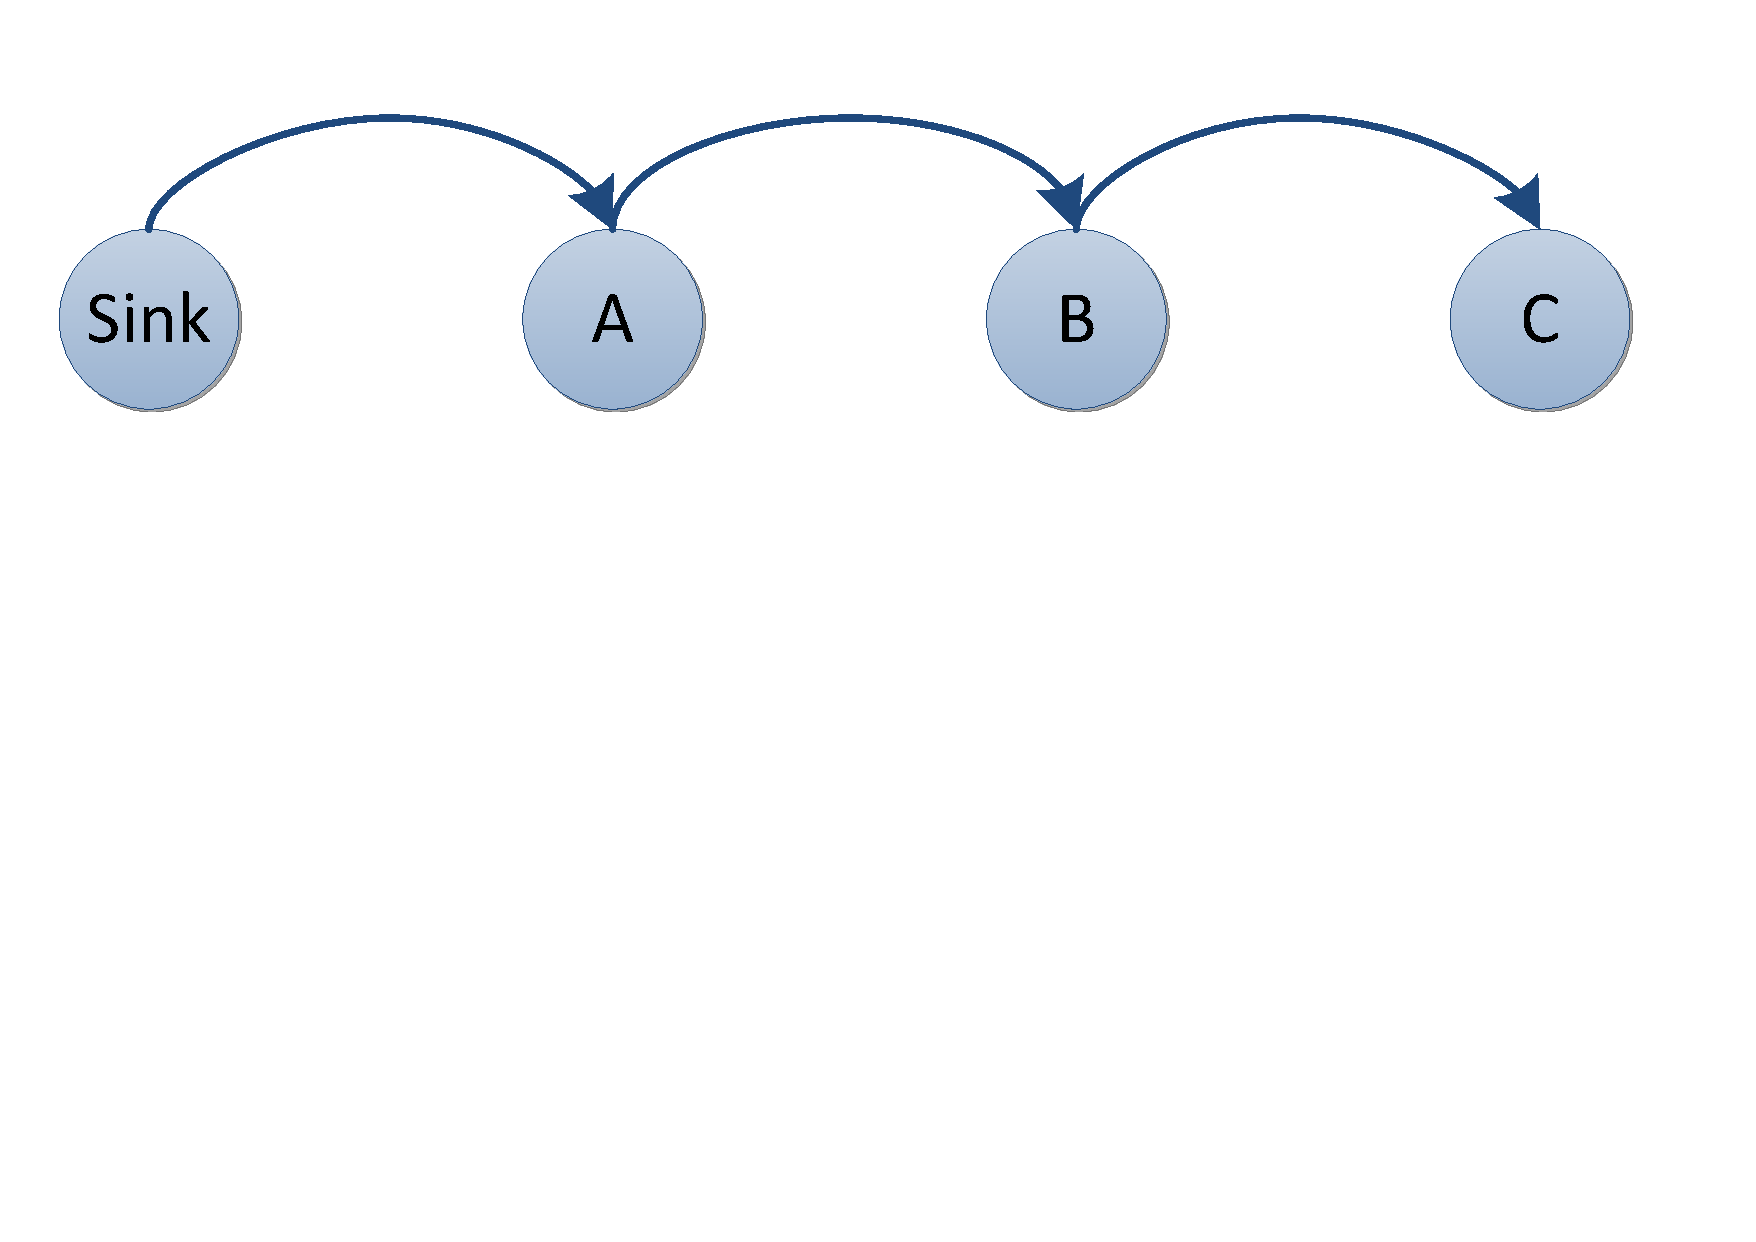
\includegraphics[height=0.6in]{images/moteRange/BetterRangeBeacon.pdf}
	\caption{A mote range 300 away would take at best 3 rounds to receive a beacon given a range of 100.}
	\label{fig:images_moteRange_rangeBeacon}
\end{figure}

To reduce this latency, HCCP uses the Roundtable Discussion to disseminate this important information.
The roundtable time can be used by motes to query for beacons, share beacons and for clusterheads to 
opt out of the clusterhead role. 

A solution to  beacon routing is to flood the network with routing information at every roundtable.
The problem with this would be the number of collisions it would create.  For instance, in a dense network,
if every node were to broadcast its beacon after receiving an update to its beacon, nearly all messages would turn
to gibberish. To prevent this, a balance of density to number of nodes beaconing must be found, or sufficient time 
must be given to the motes for each to beacon without having excessive collisions, making all collided messages overhead.


There are benefits and drawbacks to either method of sharing routing information. Sharing the beacon you received immediately
will cause collisions, but using CSMA can mitigate many of these problems.
Checking to see if the line is clear, doing a CSMA backoff if the line is busy is a simple and effective (though time consuming) way of 
dealing with most of the collisions. Collisions will still  occur, but the worst case is that some motes
might have a beacon rank that is too high.
The mote in the center does not receive a beacon from the closer motes, since the two messages collided.
Two cases can occur from here, either the center mote receives a beacon from a mote further away
from the sink, or re-requests a beacon from the surrounding motes and receives the proper rank.

Overall, the Roundtable Discussion can be a simple exchange of CSMA messages, or can
be made to do specialized tasks as needed by the network. The simulations and testbed
deployments will share routing information using simple CSMA messages.


\subsubsection{Options for Tuning the Roundtable Discussion}
\label{implementationTuning}
The Roundtable Discussion time is very expensive on the network, as all the motes
are on during this time. If a long time is chosen for the Roundtable Discussion, the 
network life will be negatively effected. If a long-lived network is desired, then 
the Roundtable Discussion should be left out all together, as long-lived networks 
are purpose built for lifespan and do not need the energy draw of the Roundtable Discussion.

If no extremely important information needs to be sent during the roundtable time, only a subset of
the motes need to be online to flood the message across the network. This too, will increase the 
lifespan of the network.

\subsection{Clusterhead Choice Timeout}
\begin{figure}[tb]
	\centering
		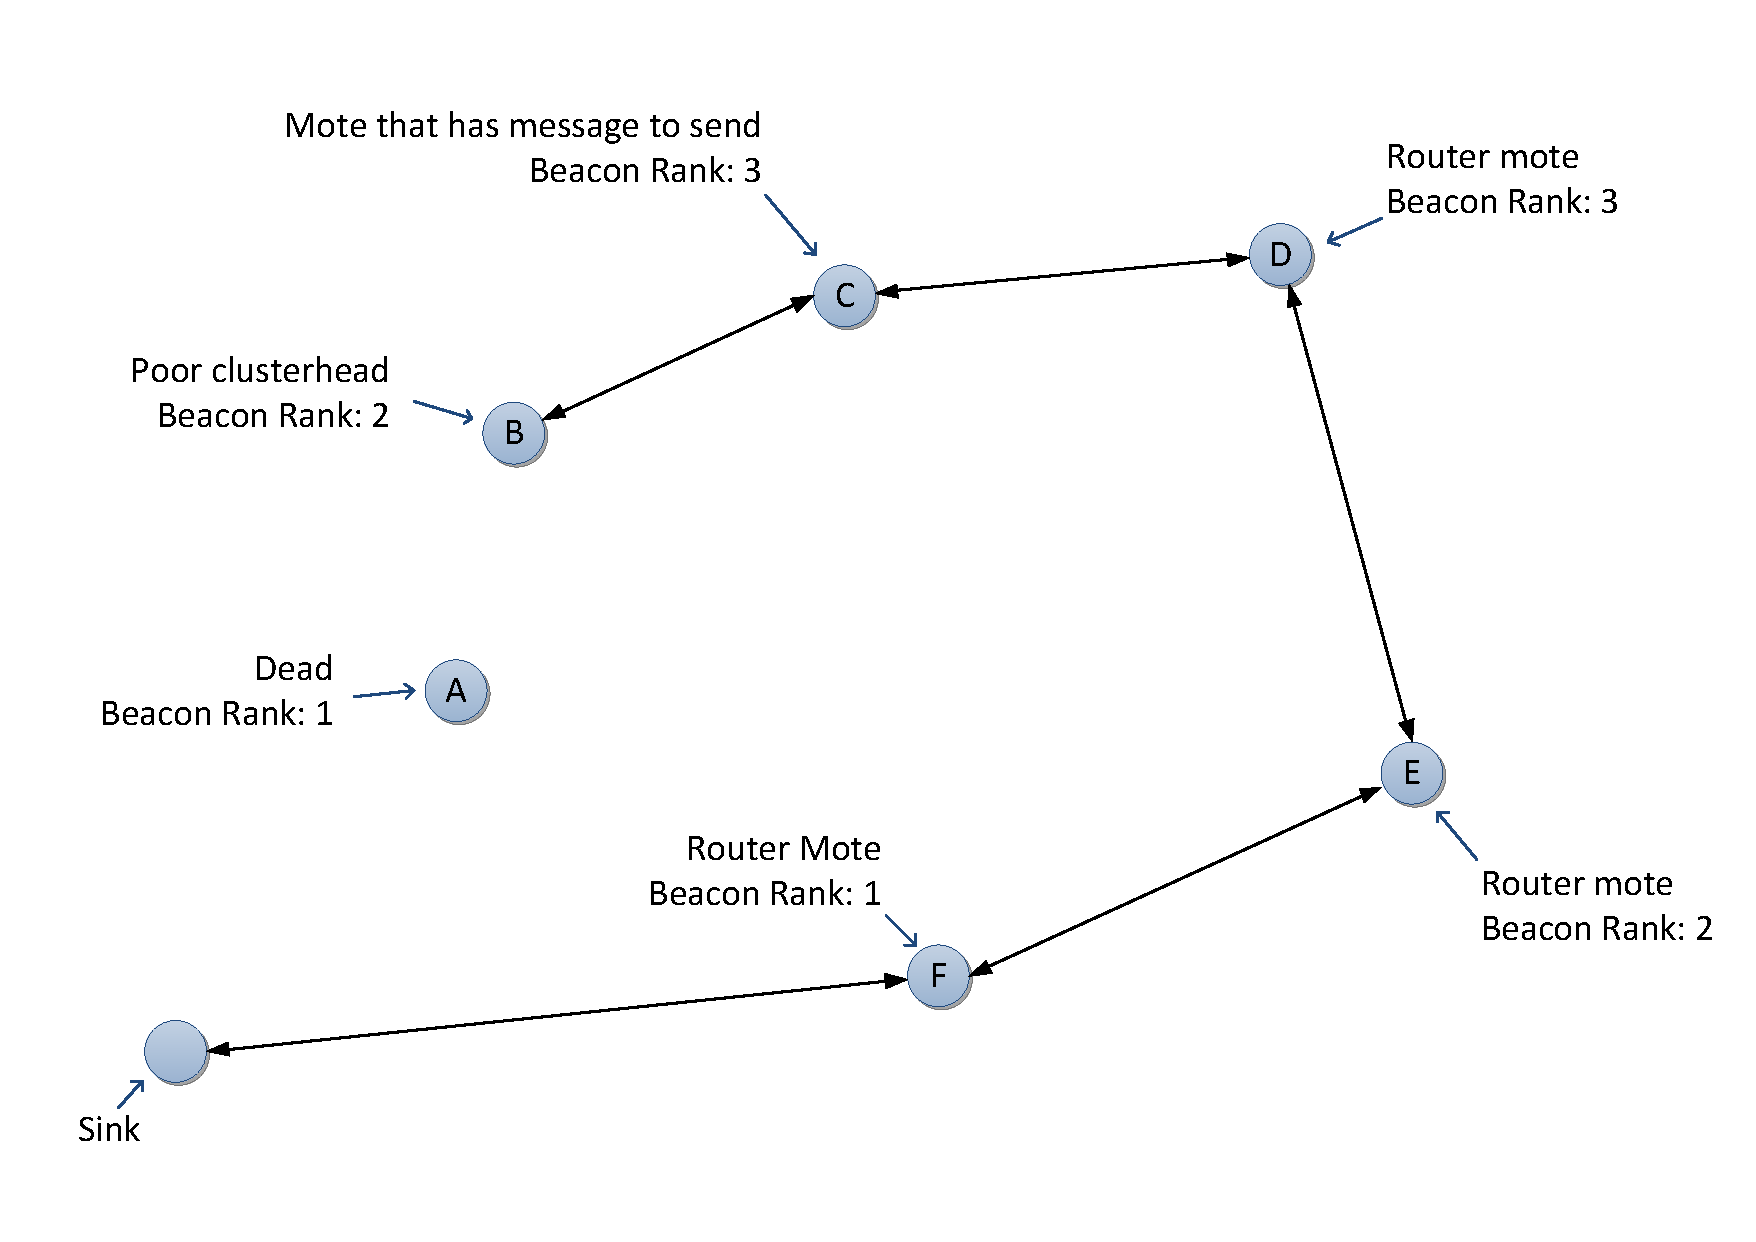
\includegraphics[width=\textwidth]{images/clusterheadChoice/BetterChooseWorseSometimes.pdf}
	\caption{Mote C would should choose mote D as a clusterhead even though mote B is closer to the sink. }
	\label{fig:image_chooseWorse}
\end{figure}



Consider the situation illustrated in Figure~\ref{fig:image_chooseWorse} where a clustermote B has a lower beacon rank than a nearby `very good' clusterhead.
The mote should choose the good clusterhead as its clusterhead over the other potential clusterheads
that may have a better beacon rank, but are significantly poorer clusterheads. 

The question that must be answered is `what is significantly poorer?'. A way to solve this problem is to use
the `Goodness Delay' timing that is already inherent in HCCP. Once a clustermote has heard a clusterhead announcement, there is a
timeout clock that starts. If another clusterhead makes an announcement before the timeout expires, and that new clusterhead 
has a lower (better) beacon rank, the mote should join that new cluster. Once the timeout has expired the quality clusterheads
that are announcing are considered significantly poorer than a known clusterhead. This is due to the `Goodness Delay' that HCCP 
uses to discover heterogeneity in the network. So, despite a mote having a lower beacon, it might not be the best clusterhead, and the 
clusterhead that is good should be used.


